\section{Producten}
Dit hoofdstuk bevat de producten waar tijdens de stage bij ConnectSB aan gewerkt wordt. Deze producten vormen de basis voor de bewijslast van de opgestelde leerdoelen die in de bijlage in het Plan van Aanpak staan.

\subsection{Content2Connect}
Content2Connect is een platform waar bedrijven grafische content in de vorm van een opdracht kunnen aanvragen. Deze bedrijven hebben dan een account waar ze de voortgang van de opdracht kunnen inzien.

In het platform bestaan vier rollen; de klant, de designer, de contactpersoon en de beheerder. De beheerder is verantwoordelijk voor het regelen van de opdrachten, het koppelen aan een designer en de klant koppelen aan een contact persoon. De designer zorgt dan dat de opdracht gemaakt wordt binnen het tijdsbestek dat aan is gegeven door de klant. Mochten er in het proces vragen of opmerkingen zijn dan handelt de contact persoon die gekoppeld zit aan deze betreffende klant deze af.

Als er een opdracht aangevraagd wordt zal er ook altijd een telefonische briefing plaatsvinden. Deze briefing wordt ook afgehandeld door de contact persoon.

De welkomst pagina van Content2Connect ziet er als volgt uit:
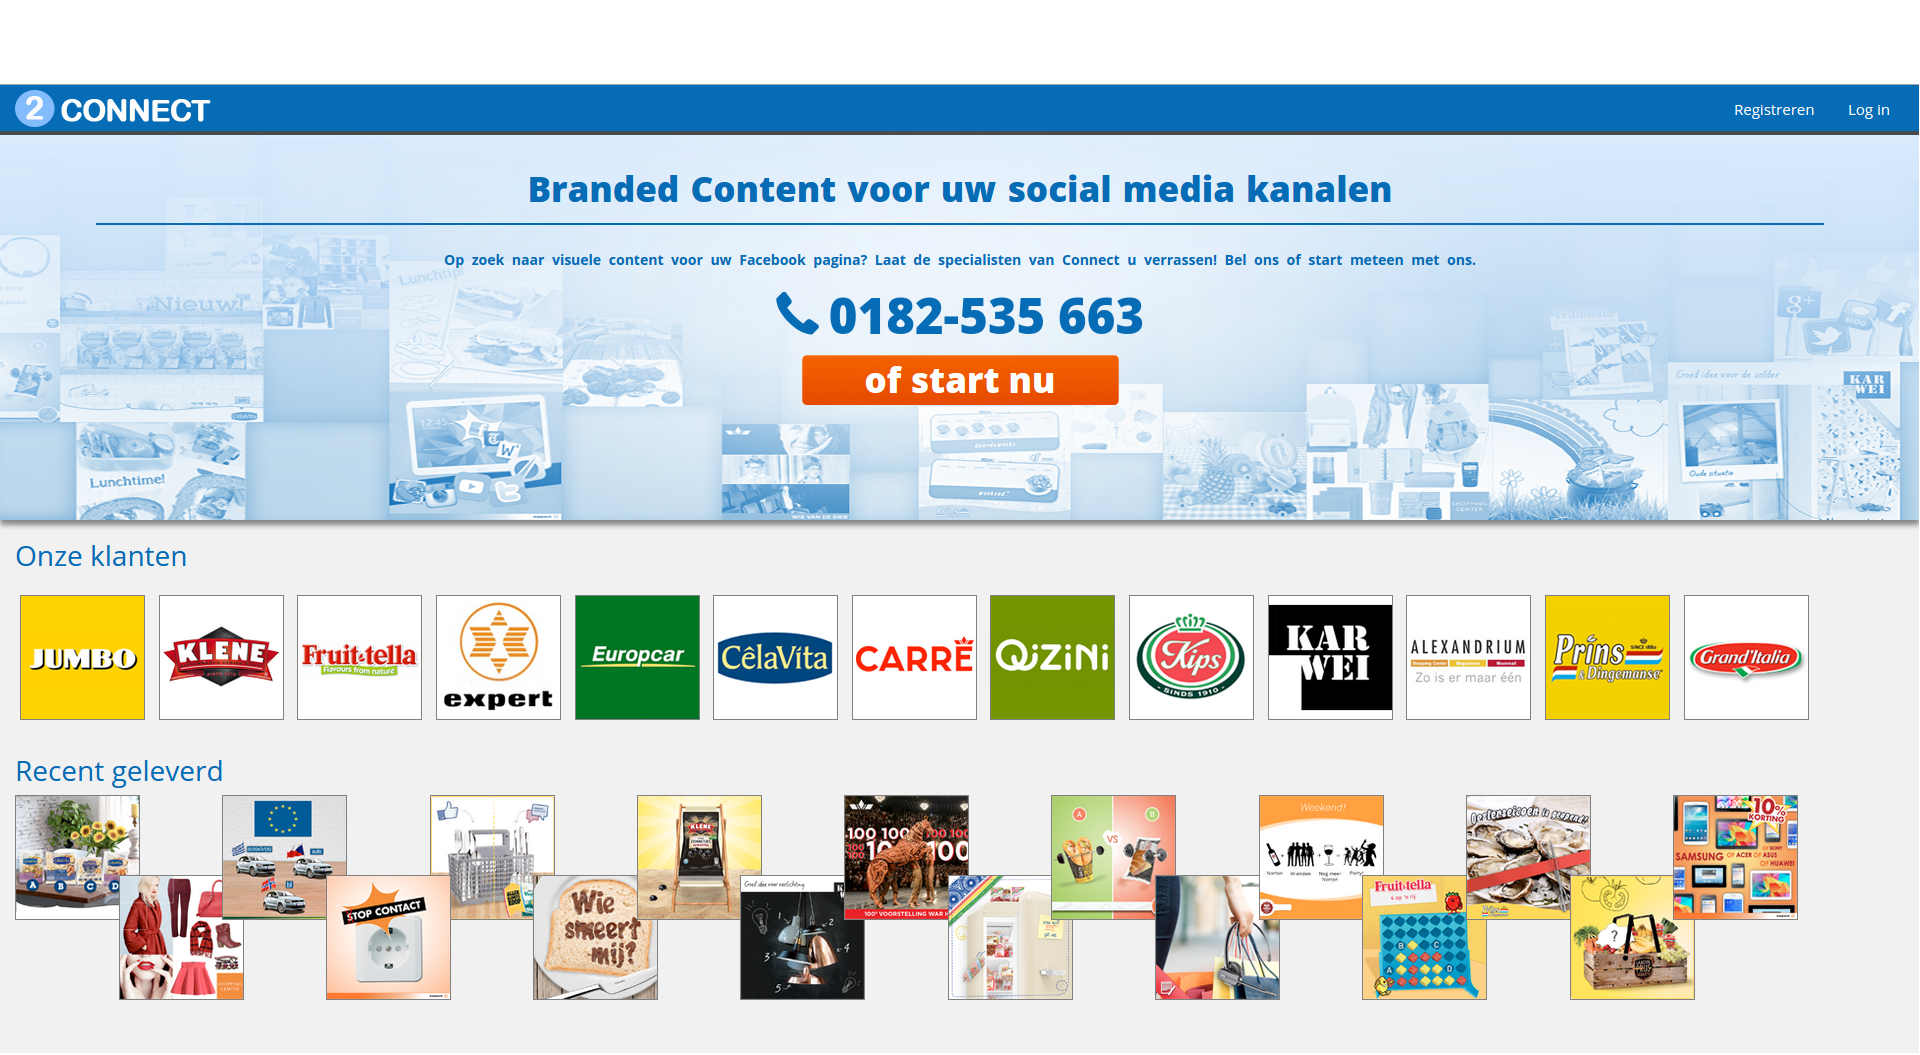
\includegraphics{content2connect}

\clearpage